% !TeX program = xelatex
% !TeX encoding = UTF-8
% !TeX spellcheck = en_US
% !BIB program = biber
%% 
%% The above lines help editors like TeXstudio to automatically choose the right tools
%% to compile your LaTeX source file. If your tool does not support these magic comments,
%% you will need to make appropriate manual choices.
%% 
%% You can safely use "pdflatex" instead of "xelatex" if you prefer the pdfLaTeX toolchain.
%% However, pdfLaTeX will not be able to deliver the professional font experience that you
%% will get with XeLaTeX. You can also safely use "lualatex" instead of "xelatex" while
%% preserving the professional font experience if you prefer the LuaLaTeX toolchain.
%% 
%% _Important_: These magic comments should be on the first lines of your source file.
%% 
%%%%%%%%%%%%%%%%%%%%%%%%%%%%%%%%%%%%%%%%%%%%%%%%%%%%%%%%%%%%%%%%%%%%%%%%%%%%%%%%

%%%%%%%%%%%%%%%%%%%%%%%%%%%%%%%%%%%%%%%%%%%%%%%%%%%%%%%%%%%%%%%%%%%%%%%%%%%%%%%%
%% 
%%            JJJJ   K                         K   UUUU         UUUU  
%%            JJJJ   KKKK                   KKKK   UUUU         UUUU  
%%            JJJJ   KKKKKK               KKKKKK   UUUU         UUUU  
%%            JJJJ      KKKKKK         KKKKKK      UUUU         UUUU  
%%            JJJJ         KKKKKK   KKKKKK         UUUU         UUUU  
%%            JJJJ            KKKKKKKKK            UUUU         UUUU  
%%    JJ     JJJJJ               KKK               UUUUU       UUUUU  
%%  JJJJJJJJJJJJJ    KKKKKKKKKKKKKKKKKKKKKKKKKKK    UUUUUUUUUUUUUUU   
%%    JJJJJJJJJ      KKKKKKKKKKKKKKKKKKKKKKKKKKK      UUUUUUUUUUU     
%% 
%% This is an example file for using the JKU LaTeX technical report template
%% for your technical report.
%% 
%% Template created by Michael Roland (2021)
%% 
%%%%%%%%%%%%%%%%%%%%%%%%%%%%%%%%%%%%%%%%%%%%%%%%%%%%%%%%%%%%%%%%%%%%%%%%%%%%%%%%

%%%%%%%%%%%%%%%%%%%%%%%%%%%%%%%%%%%%%%%%%%%%%%%%%%%%%%%%%%%%%%%%%%%%%%%%%%%%%%%%
%% 
%% Document class: This is a koma-script article.
%% 
\documentclass[a4paper,oneside,10pt,ngerman,english]{scrartcl}
%% 
%% The comma-separated list in square brackets are class options.
%% Useful options that you might want to use:
%% 
%% Paper size:
%%  * a4paper ... A4 paper size
%% 
%% Optimize for single-sided or double-sided printing:
%%  * oneside ... single-sided
%%  * twoside ... double-sided
%% 
%% Base font size:
%%  * 10pt ... 10-pt font is used for normal text
%%  * 11pt ... 11-pt font is used for normal text
%% 
%% Define document languages (the last specified language becomes the document default
%% language):
%%  * ngerman ... German
%%  * english ... English
%%  * ...
%% 
%% Alternate document classes: The JKU report template supports the koma-script classes
%% `scrartcl', `scrreprt' and `scrbook'. The article class `scrartcl' is well-suited
%% for a typical technical report. However, `scrbook' or `scrreprt' may be better
%% suited for longer reports since they permit structuring your work in chapters.
%%  
%% _Important_: The document class should be the first line of LaTeX code in your main
%% source file. Do not place anything but comments / magic comments above that line (unless
%% you really know what you are doing).
%% 
%%%%%%%%%%%%%%%%%%%%%%%%%%%%%%%%%%%%%%%%%%%%%%%%%%%%%%%%%%%%%%%%%%%%%%%%%%%%%%%%

%%%%%%%%%%%%%%%%%%%%%%%%%%%%%%%%%%%%%%%%%%%%%%%%%%%%%%%%%%%%%%%%%%%%%%%%%%%%%%%%
%% 
%% Treat input files as UTF-8 encoded. Make sure to always load this when you use pdfLaTeX
%% so that pdfLaTeX knows how to read and interpret characters in this source file.
%% 
\usepackage[utf8]{inputenc}
%% 
%%%%%%%%%%%%%%%%%%%%%%%%%%%%%%%%%%%%%%%%%%%%%%%%%%%%%%%%%%%%%%%%%%%%%%%%%%%%%%%%

%%%%%%%%%%%%%%%%%%%%%%%%%%%%%%%%%%%%%%%%%%%%%%%%%%%%%%%%%%%%%%%%%%%%%%%%%%%%%%%%
%% 
%% Use the JKU LaTeX technical report template for this document.
%% 
\usepackage[techreport,fancyfonts]{jkureport}
%% 
%% The comma-separated list in square brackets are theme options. Useful options that you
%% might want to use:
%% 
%% Document type:
%%  * phdthesis     ... PhD thesis.
%%  * mathesis      ... Master's thesis.
%%  * diplomathesis ... Diploma thesis.
%%  * bathesis      ... Bachelor's thesis.
%%  * seminarreport ... Seminar report.
%%  * techreport    ... Technical report.
%% 
%% Color scheme selection options:
%%  * JKU  ... Use JKU (gray) color scheme (this is the default if no scheme is selected).
%%  * BUS  ... Use Business School color scheme.
%%  * LIT  ... Use Linz Institute of Technology color scheme.
%%  * MED  ... Use MED faculty color scheme.
%%  * RE   ... Use RE faculty color scheme.
%%  * SOE  ... Use School of Education color scheme.
%%  * SOWI ... Use SOWI faculty color scheme.
%%  * TNF  ... Use TNF faculty color scheme.
%% 
%% Space-efficient monospace font options (requires XeTeX/LuaTeX):
%%  * compactmono   ... Use condensed fixed-width font everywhere.
%%  * nocompactverb ... Do not use condensed fixed-width font for verbatim and listings.
%% 
%% Style-breaking options:
%%  * noimprint      ... Do not insert imprint on title pages.
%%  * nojkulogo      ... Do not insert JKU & K logos on title pages.
%%  * capstitle      ... Set document title in capital letters.
%%  * nofancyfonts   ... Do not use custom TTF fonts with XeTeX/LuaTeX / supress pdfLaTeX warning.
%%  * equalmargins   ... Decrease the outer page margin to have both page margins of equal size
%%                       (the additional outer margin is intentional and to be used for
%%                       anotations; equalmargins also causes the text width to be
%%                       significantly larger than optimal for reading).
%% 
%% Experimental options:
%%  * mathastext ... Use standard document fonts (enhanced with symbols from Fira Math font
%%                   when using XeTeX/LuaTeX) in math mode.
%% 
%% Advanced options:
%%  * noautopdfinfo     ... Do not automatically try to add pdfinfo with hyperref from document
%%                          metadata fields.
%%  * logopath={<path>} ... Set the path where the theme can find its own logo resources. This
%%                          should typically be a relative path and the default is `./logos'.
%%  * fontpath={<path>} ... Set the path where the theme can find its own font resources. This
%%                          should typically be a relative path and the default is `./fonts'.
%% 
%% Hint: Boolean options can be used in the forms `option' or `option=true' the enable the
%% option and `nooption' or `option=false' to disable the option.
%% 
%%%%%%%%%%%%%%%%%%%%%%%%%%%%%%%%%%%%%%%%%%%%%%%%%%%%%%%%%%%%%%%%%%%%%%%%%%%%%%%%

%%%%%%%%%%%%%%%%%%%%%%%%%%%%%%%%%%%%%%%%%%%%%%%%%%%%%%%%%%%%%%%%%%%%%%%%%%%%%%%%
%% 
%% This is the place where you can load additional packages. If you want to load
%% a package `biblatex', you would use the command `\usepackage{biblatex}'.
%% 

\usepackage{csquotes}
\usepackage[backend=biber,citestyle=numeric,sortcites=true,maxcitenames=2,style=ACM-Reference-Format]{biblatex}
\setcounter{biburlnumpenalty}{100} %% reducing biburl* penalties typically improves URL placement in bibliography
\setcounter{biburllcpenalty}{100}
\setcounter{biburlucpenalty}{100}
\usepackage{todonotes}
\usepackage{import}
\usepackage{amsfonts}
\usepackage{subfigure}
%\usepackage{acronym}

%% 
%%%%%%%%%%%%%%%%%%%%%%%%%%%%%%%%%%%%%%%%%%%%%%%%%%%%%%%%%%%%%%%%%%%%%%%%%%%%%%%%

%%%%%%%%%%%%%%%%%%%%%%%%%%%%%%%%%%%%%%%%%%%%%%%%%%%%%%%%%%%%%%%%%%%%%%%%%%%%%%%%
%% 
%% Bibliography data files.
%% 

\addbibresource{references.bib}

%% 
%%%%%%%%%%%%%%%%%%%%%%%%%%%%%%%%%%%%%%%%%%%%%%%%%%%%%%%%%%%%%%%%%%%%%%%%%%%%%%%%

\begin{document}
%%%%%%%%%%%%%%%%%%%%%%%%%%%%%%%%%%%%%%%%%%%%%%%%%%%%%%%%%%%%%%%%%%%%%%%%%%%%%%%%
%% 
%% Report information and title page
%% 

%% Command \title{title}: sets the title of your report
\title{Data-Driven Insights for Intelligent Transport Systems: From Vehicle Perception to Human Interaction}

%% Command \titleshort{short title}: sets an abbreviated version of the report title for page heads
%\titleshort{Optional space for your abbreviated title}

%% Command \subtitle{subtitle}: sets the subtitle for seminar/technical reports (not used for theses)
\subtitle{Pre-defense report\\%
    \usekomafont{subtitlesmall}%
    \hfill\\%
    Supervisor: Prof. Dr. Cristina Olaverri-Monreal\\
    Co-Supervisor: Prof. Dr. Jonas Sj{\"o}berg\\
    \hfill\\%
}

%% Command \author{name}: sets the author name(s); separate multiple authors with \and; use \prefix{}
%%   and \suffix{} to add academic titles and suffixes (if needed); use \affiliation{} to add an
%%   affiliation, use \authornewline to add line breaks (e.g. to separate authors from contact
%%   information), use \authormail{}, \authorweb{}, \authorphone{} and \authorfax{} to add contact
%%   information)
\author{%
    Novel Certad
    \affiliation{Department Intelligent Transport Systems}
    \authornewline
    \authorphone{+43 732 2468-XXXX}
    \authormail{novel.certad\_hernandez@jku.at}
    \authorweb{https://jku.at/its}
    \authornewline
}

%% Command \date{YYYY-MM-DD}: set the day of publication (defaults to today)
%\date{2020-04-09}

%% Command \partnerlogo{filename}: use filename as partnerlogo, filename may be blank to disable the logo
%\partnerlogo{logos/ins}

%% Command \revisionblock{text}: set the document revision block on the title page
\revisionblock{Space for your revision block, acknowledgements, etc.}

%% Command \reportnumber{number}: set the report number
%\reportnumber{Space for your report number}

%% Command \setbottommark{text}: set the bottom mark (in document footer)
%\setbottommark{Space for your bottom mark}

%% Command \abstract{text}: set the document abstract on the title page
\abstract{Space for your (short) abstract.}

%% Command \keywords{text}: set the document keywords
%\keywords{Space for your comma-separated keywords}


%% Finally, print the title page using the above information:
\maketitle
%% 
%%%%%%%%%%%%%%%%%%%%%%%%%%%%%%%%%%%%%%%%%%%%%%%%%%%%%%%%%%%%%%%%%%%%%%%%%%%%%%%%

%%%%%%%%%%%%%%%%%%%%%%%%%%%%%%%%%%%%%%%%%%%%%%%%%%%%%%%%%%%%%%%%%%%%%%%%%%%%%%%%
%% 
%% Add a table of contents
%% 

%% Make sure to start the table of contents on a new odd page (odd is only relevant in twoside layout)
\cleardoubleoddpage
%% Print the table of contents
\tableofcontents

%% Make sure to start the list of acronyms on a new odd page (odd is only relevant in twoside layout)
%\cleardoubleoddpage
%% Include list of acronyms (optional and often not necessary)
%\import{./}{acronyms}

%% 
%%%%%%%%%%%%%%%%%%%%%%%%%%%%%%%%%%%%%%%%%%%%%%%%%%%%%%%%%%%%%%%%%%%%%%%%%%%%%%%%

%%%%%%%%%%%%%%%%%%%%%%%%%%%%%%%%%%%%%%%%%%%%%%%%%%%%%%%%%%%%%%%%%%%%%%%%%%%%%%%%
%% 
%% Abstract: Instead of an abstract on the title page (see \abstract{...}), you
%% sometimes want to add an abstract as its own unnumbered section.
%% 

%% (Optionally) let the abstract start on a new odd page (odd is only relevant in twoside layout)
\cleardoubleoddpage

\addsec{Abstract}

Space for your abstract.


%% 
%%%%%%%%%%%%%%%%%%%%%%%%%%%%%%%%%%%%%%%%%%%%%%%%%%%%%%%%%%%%%%%%%%%%%%%%%%%%%%%%

%%%%%%%%%%%%%%%%%%%%%%%%%%%%%%%%%%%%%%%%%%%%%%%%%%%%%%%%%%%%%%%%%%%%%%%%%%%%%%%%
%% 
%% Add your report sections ...
%% 

%% (Optionally) let the main sections start on a new odd page (odd is only relevant in twoside layout)
\cleardoubleoddpage

\section{Introduction}
\label{sec:introduction}

A single-column 4 page report has to be submitted to the chair of PhD affairs (Prof. Josef Küng for candidates in Computer Science and Prof. Johannes Fürnkranz for candidates in Artificial Intelligence) two weeks before the pre-defense in order for the chair and examiner to prepare questions. They will get the report before the pre-defense starts and should prepare one or two questions each.

The report should contain 3 parts:
scientific part (maximum 2 pages, 11pt font, standard margins)
- motivation (for the general audience)
- approach, results, future work
progress part (maximum 1 page, 11pt font, standard margins)
- published/submitted/planned papers or other output (including talks, SW, systems, stay abroad, organized events, awards etc)
- description of the candidate's contributions, impact
references (1 page, but actually without page limit)



\section{Scientific Part}
\label{sec:science}

\subsection{motivation}



% This dissertation explores critical aspects of **automated driving systems (ADS)**, ranging from the fundamental challenges of **road marking (RM) 
% visibility** to the complexities of **real-world vehicle and pedestrian interactions**.  Initial research focused on the impact of RM materials on 
% their visibility for machine vision, demonstrating that **different RM types exhibit varying performance under diverse conditions, including dry, 
% wet, day, night, and glare**. The study quantified how these visibility variations affect the performance of camera-based ADAS, revealing failure 
% points in lane detection and trajectory planning. This foundational work highlights the crucial role of **road infrastructure quality** in enabling 
% reliable autonomous navigation. Additionally, the research extended to the **use of LiDAR sensors** in RM detection, demonstrating that 
% **reflectivity data provides superior results compared to intensity data alone** when segmenting RMs from point clouds.

% Building on the sensor-level understanding, the research then examined how to extract meaningful information about the behavior of road users. Applying 
% the **IEEE Standard 2846-2022** methodology, the work explored how to extract kinematic data from real-world scenarios, and determine safety-relevant 
% assumptions about road user behavior. This involved analyzing realistic driving data to establish **kinematic boundaries** for other road users, offering 
% a basis for ADS to make informed decisions. In addition, a novel dataset was created that integrates multi-modal sensor data, including direct access to 
% the vehicle bus, **providing a comprehensive view of diverse traffic scenarios in Germany**.  This **IAMCV dataset** includes data from highways, country 
% roads, roundabouts, and intersections, which is crucial for the training and validation of ADS algorithms.


% Finally, the dissertation addresses the complexities of **vehicle-to-pedestrian (V2P) interactions**, evaluating the effectiveness of different warning 
% systems for distracted pedestrians. This research provided empirical evidence that **V2P technology can significantly improve pedestrian safety**, 
% specifically through a comparative study with traditional auditory warning systems. The experimental results highlighted how **pedestrian behavior changes 
% in response to visual or auditory alerts**, accounting for varying levels of distraction. The work thus provides insights on the development of effective 
% alerts for vulnerable road users within the context of shared urban environments. Overall, these interconnected research threads highlight that **the safety 
% and reliability of ADS is determined by the complex interactions between infrastructure, sensors, and all road users**.
The pursuit of fully autonomous vehicles (AVs) represents one of the most ambitious technological challenges in modern transportation. A key stepping stone toward achieving this vision is the gradual development and deployment of Advanced Driver Assistance Systems (ADAS). ADAS technologies, while currently limited in their capabilities, serve as a critical intermediary, bridging the gap between manually driven vehicles and fully autonomous systems. By incrementally enhancing the level of autonomy through increasingly sophisticated ADAS, these systems allow vehicles to perform specific tasks in controlled operational design domains (ODDs). This approach not only enhances road safety but also provides a framework for the eventual realization of fully autonomous vehicles.

This dissertation explores critical aspects of automated driving systems (ADS), ranging from the fundamental challenges of road marking (RM) visibility to the complexities of real-world vehicle and pedestrian interactions. Initial research focused on the impact of RM materials on their visibility for machine vision, demonstrating that different RM types exhibit varying performance under diverse conditions, including dry, wet, day, night, and glare. The study quantified how these visibility variations affect the performance of camera-based ADAS, revealing failure points in lane detection and trajectory planning. This foundational work highlights the crucial role of road infrastructure quality in enabling reliable autonomous navigation. Additionally, the research extended to the use of LiDAR sensors in RM detection, demonstrating that reflectivity data provides superior results compared to intensity data alone when segmenting RMs from point clouds.

Building on the sensor-level understanding, the research then examined how to extract meaningful information about the behavior of road users. Applying the IEEE Standard 2846-2022 methodology, the work explored how to extract kinematic data from real-world scenarios, and determine safety-relevant assumptions about road user behavior. This involved analyzing realistic driving data to establish kinematic boundaries for other road users, offering a basis for ADS to make informed decisions. In addition, a novel dataset was created that integrates multi-modal sensor data, including direct access to the vehicle bus, providing a comprehensive view of diverse traffic scenarios in Germany. This IAMCV dataset includes data from highways, country roads, roundabouts, and intersections, which is crucial for the training and validation of ADS algorithms.

Finally, the dissertation addresses the complexities of vehicle-to-pedestrian (V2P) interactions, evaluating the effectiveness of different warning systems for distracted pedestrians. This research provided empirical evidence that V2P technology can significantly improve pedestrian safety, specifically through a comparative study with traditional auditory warning systems. The experimental results highlighted how pedestrian behavior changes in response to visual or auditory alerts, accounting for varying levels of distraction. These findings contribute valuable insights into the development of effective alerts for vulnerable road users within the context of shared urban environments. Overall, the interconnected research threads emphasize that the safety and reliability of ADS are determined by the complex interactions between infrastructure, sensors, and all road users.



\subsection{Approach}
\subsection{Results}
\subsection{Future work} 


\section{Progress}
\label{sec:progress}




\section{Example}
\label{sec:example}

This is an example for another section in your thesis.
It should primarily show you some basic \LaTeX\ tricks.
For instance, \ref{sec:introduction} references to your introduction.
You can also embed figures, tables, etc.\ in your work.
\ref{fig:learningcenter} is an example for a figure (i.e.\ photos, diagrams, and other artwork).
Note that figures (just like tables, see) are floating elements.
They are either placed at the top or bottom of a page (or sometimes stand on their own page), but not in between your text.
You can influence their placement with the placement modifiers ``t'', ``b'', and ``p''.
Bottom placement (``b'') is sometimes more tricky, as \LaTeX\ does not consider this nice in some situations.
You can convince \LaTeX\ to honor your placement expectation with ``!b'' then.
Since you do not place figures/tables in between your running text, you always need to reference them by their label (e.g.\ \ref{fig:learningcenter}).
\begin{figure}[!b]
\centering
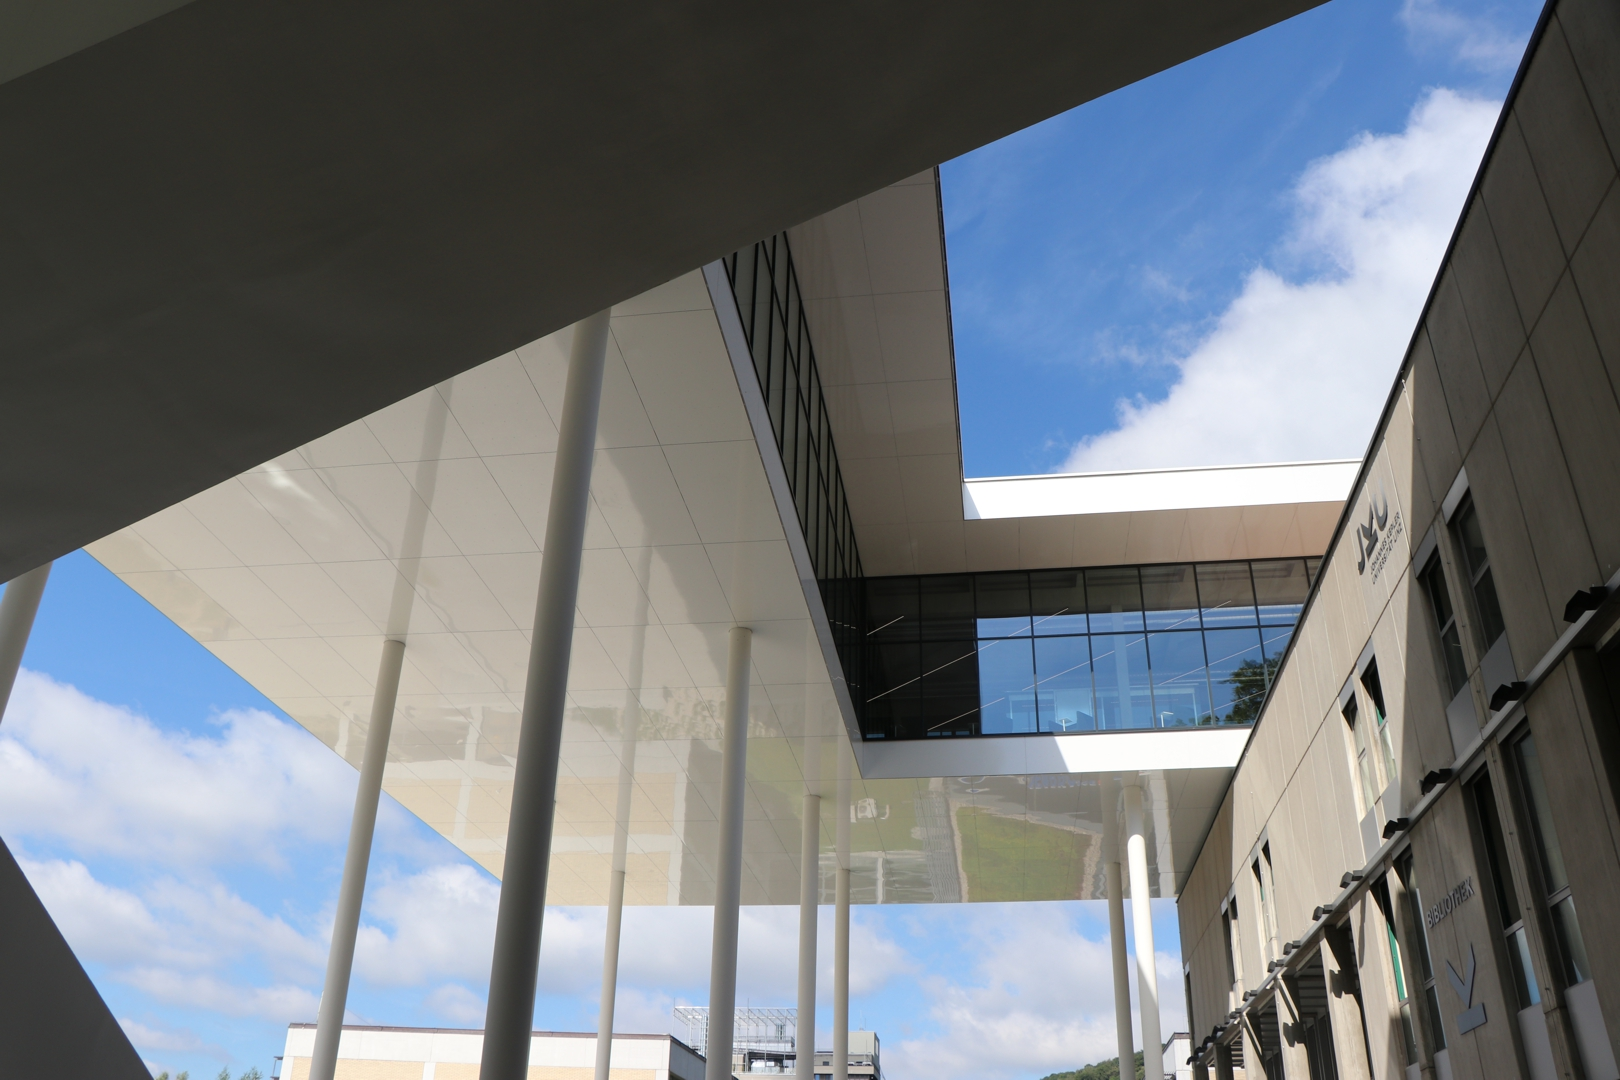
\includegraphics[width=\linewidth]{images/jku_learningcenter}
\caption{
    A figure. Be aware that figures have their caption below the artwork
}\label{fig:learningcenter}
\end{figure}


\cite{certad2022}
\cite{certad2023}
\cite{iamcv_paper}
\cite{its-vehicle}
\cite{certad2024irf}

\cite{certad2025swarco}
\cite{certad2025}

\cite{dora}
\cite{iamcv_dataset}
\cite{morales2022}
\cite{morales2023}
\cite{delre2025}



\section{Conclusion}
\label{sec:conclusion}

Space for your summary, central conclusions, and an outlook on potential future work.


%% 
%%%%%%%%%%%%%%%%%%%%%%%%%%%%%%%%%%%%%%%%%%%%%%%%%%%%%%%%%%%%%%%%%%%%%%%%%%%%%%%%

%%%%%%%%%%%%%%%%%%%%%%%%%%%%%%%%%%%%%%%%%%%%%%%%%%%%%%%%%%%%%%%%%%%%%%%%%%%%%%%%
%% 
%% Print the bibliography
%% 
%% (Optionally) let the bibliography start on a new odd page (odd is only relevant in twoside layout)
%\cleardoubleoddpage
\printbibliography
%% 
%%%%%%%%%%%%%%%%%%%%%%%%%%%%%%%%%%%%%%%%%%%%%%%%%%%%%%%%%%%%%%%%%%%%%%%%%%%%%%%%

%% Begin with the appendix part (all further sections will be appendices)
\appendix

%%%%%%%%%%%%%%%%%%%%%%%%%%%%%%%%%%%%%%%%%%%%%%%%%%%%%%%%%%%%%%%%%%%%%%%%%%%%%%%%
%% 
%% Add your appendix sections ...
%% 

%% Make sure to start the appendix on a new odd page (odd is only relevant in twoside layout)
%\cleardoubleoddpage
\section{An Appendix}
\label{app:an-appendix}

Space for an appendix.
You can have more than one appendix section.
Appendices are, of course, optional.


%% 
%%%%%%%%%%%%%%%%%%%%%%%%%%%%%%%%%%%%%%%%%%%%%%%%%%%%%%%%%%%%%%%%%%%%%%%%%%%%%%%%

\cleardoubleoddpage

\end{document}
\endinput
